\typeout{ ====================================================================}
\typeout{ this is file mef.tex, created at 22-Feb-2015               }
\typeout{ maintained by Gustavo Rabello dos Anjos                             }
\typeout{ e-mail: gustavo.rabello@gmail.com                                   }
\typeout{ ====================================================================}


\section{MÉTODO DE ELEMENTOS FINITOS}

No método de elementos finitos, o domínio é divido em um número
de sub-domínios finitos conhecidos como elementos.  Uma simples função é
utilizada para caracterizar a variação de cada variável dentro do
elemento.  Esta funcão recebe o nome \emph{função de forma}.  A
justaposição da variação das variáveis em cada elemento é usada
para descrever todo o campo do fluido.  

Podem-se considerar como caracterísicas principais do método dois
conceitos:

\begin{itemize}
	\item a utilização da forma fraca, ou variacional, do problema;
	\item solução aproximada da equação variacional através do uso de
	funções dos elementos finitos.
\end{itemize}

A forma fraca é resultado da ponderação da equação original em sua forma
forte (forma diferencial inicial, não alterada) em um domínio qualquer.  É
necessário encontrar uma solução tentativa $u$ que satisfaça a seguinte
expressão:

\begin{equation}
	\int_{\Omega} (\frac{du}{dx})^2 \, dx < \infty
\label{eq:fem_weak1}
\end{equation}\hspace{0.5cm}

Uma função que satisfaça a Eq.~(\ref{eq:fem_weak1}) é chamda de
\textbf{\textit{função $H^1$}}. 
Uma outra classe de funções é necessária, são as chamadas
\textbf{\textit{funções peso}}, que são funções do tipo $H^1$ com uma
característica a mais.  Para o caso de problema de Dirichlet, no contorno 
do domínio elas são nulas.  Utilizando estas definições, pode-se provar
\cite{hughes1987} que a forma forte da equação de difusão em 1D
\begin{align}
	\frac{d}{dx} \bigg( k\frac{du}{dx} \bigg) -f 
	= 
	0&
	\qquad
	\text{em}
	\qquad
	\Omega
	\\
	&u=u_1 \qquad \text{em} \Gamma_1
	\\
	&u=u_2 \qquad \text{em} \Gamma_2
\label{eq:fem1}
\end{align}

\noindent é equivalente à sua forma fraca representada pela Eq.~(\ref{eq:fem1}) 
depois de passar por integração por partes do termo difusivo:
\textbf{Achar $u \in H^1_\Gamma$ tal que, para qualquer $W \in H^1_0$}

\begin{equation}
	\int_{\Omega}w \bigg[ k \frac{d}{dx} \bigg( \frac{du}{dx} \bigg) -f
	\bigg]
	= 0 \longrightarrow
	\int_{\Omega} k \frac{dw}{dx} \frac{du}{dx} d\Omega
	= 
	\int_{\Omega} wf \, d\Omega + c.c.
	\label{eq:fem2}
\end{equation}

\noindent $w$ representa a função peso e $\Omega$ representa o domínio
do problema, que para esse caso-exemplo está contido no intervalo
fechado, $\Omega \in [0,1]$.  

Até esse momento não houve quaisquer aproximações e o problema ainda não
foi discretizado.  A seguir, através do método de Galerkin serão 
obtidas soluções aproximadas para a equação diferencial em questão. 

Considerando $\Omega$ o domínio do problema e $\Omega^e$ o domínio do
elemento, então:

\begin{equation}
	\bigcup_{n=1}^{N} \Omega^e 
	= 
	\Omega\text{;}
	\qquad
	\Omega^i \cap \Omega^j = 0\text{;}
	\qquad
	i \neq j
\label{eq:malha1}
\end{equation}\hspace{0.5cm}

\noindent sendo a malha formada por $N$ elementos que podem ter dimensões
características diferentes.  Considere ainda que para cada elemento da
malha está definida uma família de funções 

\begin{equation}
	N^e 
	= 
	\big [ 
	N_1^e \cdots N_S^e 
	\big] 
\label{eq:fem3}
\end{equation}\hspace{0.5cm}

\noindent onde $S$ representa o número de nós que definem o elemento.
Para um elemento linear (Fig.~\ref{fig:elemento1}a), $S=2$, já para um
elemento quadrático 1D (Fig.~.\ref{fig:elemento1}b), $S=3$.  

\begin{figure}[h]
	\centering
		 %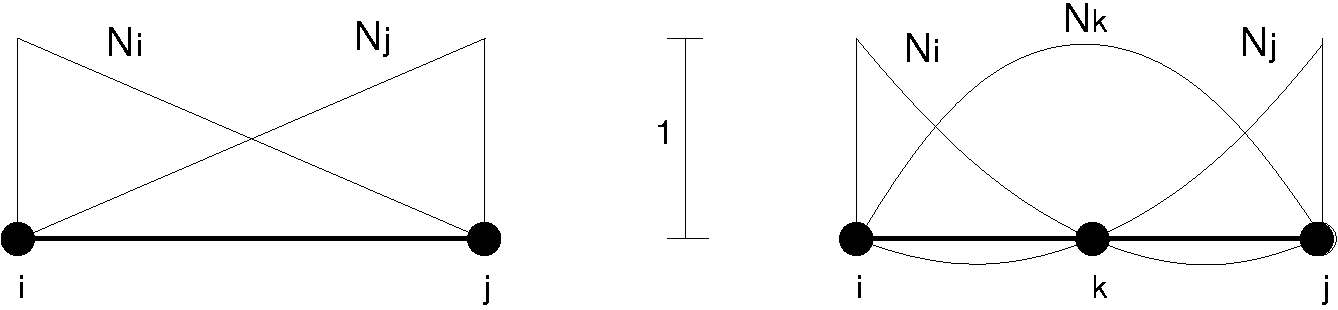
\includegraphics[scale=0.6]{figs/elem1.pdf}
		 \caption{Representação de elementos unidimensionais linear à
		 esquerda e quadrático à direita.} 
	\label{fig:elemento1}
\end{figure}

A diferença entre os dois elementos está no grau do polinômio
interpolador.  Para o elemento linear, a função interpoladora apresenta
grau 1 enquanto que no elemento quadrático, a função interpoladora é de
grau 2. Elementos de baixa ordem apresentam custo computacional baixo
comparado aos de mais alta ordem, entretanto não oferecem a mesma
precisão numérica. Considerando que as funções interpolação são da forma

\begin{equation}
	u^e(x) 
	= 
	\sum_n u_j(x) N^e_j
\end{equation}\hspace{0.5cm}
\begin{equation}
	w^e(x) 
	= 
	\sum_n w_i(x) N^e_i
\end{equation}\hspace{0.5cm}

\noindent e aplicando-se o método de Galerkin na forma fraca da equação 
de difusão, chega-se a:

\begin{equation}
	\sum_e \int_{\Omega^e} \sum_{i,j \in e} \alpha \frac{dN^e_i}{dx}
	\frac{dN^e_j}{dx} \, u_j d\Omega  
	=
	\sum_e \int_{\Omega^e} \sum_{i \in e} N_i^e f \, d\Omega + \text{c.c.} 
\label{eq:galerkin1D}
\end{equation}\hspace{0.5cm}

\noindent rearranjando os termos com somatório dentro da integral, a
equação define um sistema linear do tipo

\begin{equation}
	\mathbf{K}u = \mathbf{f} 
	\label{eq:sistemalinear}
\end{equation}\hspace{0.5cm}

\noindent onde $u$ tem como componentes os valores nodais $u_n$, a
matriz $\mathbf{K}$ e o vetor $\mathbf{f}$ representados por uma
montagem especial conhecida com \emph{Assembling}:

\begin{equation}
	\mathbf{K} = \overset{nele}{\underset{e=1}{\mathcal{A}}} k^e; \quad
	\mathbf{f} = \overset{nele}{\underset{e=1}{\mathcal{A}}} f^e
\end{equation}

\noindent e $\mathcal{A}$ é o operador montagem. A matriz $k^e$ e o vetor $f^e$
são definidos por

\begin{equation}
	k_{i,j} = \int_{\Omega^e}\alpha \frac{dN_i^e}{dx} \frac{dN_j^e}{dx}
	d\Omega
	\qquad
	i,j=2
\end{equation}\hspace{0.5cm}

\begin{equation}
	f_{i} = \int_{\Omega^e} N_i^e f \, d\Omega
	\qquad \qquad
	i=2
\end{equation}

\noindent As integrais acima podem ser resolvidas analiticamente ou
através de métodos numéricos.  Em elementos finitos, o método numérico
mais popular é a quadratura gaussiana, porém, para o caso
unidimensional, o resultado analítico dessas integrais é simples.
Dependendo do tipo de função de forma escolhido, o erro de aproximação
diminui.  Para este caso, considera-se o elemento linear representado
por:

\begin{align}
	&N_i = 1 - \frac{x-x_i}{h}
	\\
	&N_j = \frac{x - x_j}{h} 
\end{align}

\noindent onde $h$ representa o tamanho característico do elemento,
obtem-se:

\begin{gather*}
	k^e 
	= 
	\frac{\alpha}{h}\begin{bmatrix}1 & -1 \\ -1 &1\end{bmatrix}
	\qquad \text{e} \qquad
	f^e 
	=  
	h\begin{bmatrix}1 \\ 1\end{bmatrix}
\end{gather*}

\noindent Realizando o procedimento de \emph{Assembling} chega-se ao
sistema linear (Eq.~\ref{eq:sistemalinear}):

\begin{figure}[h]
	\centering
		%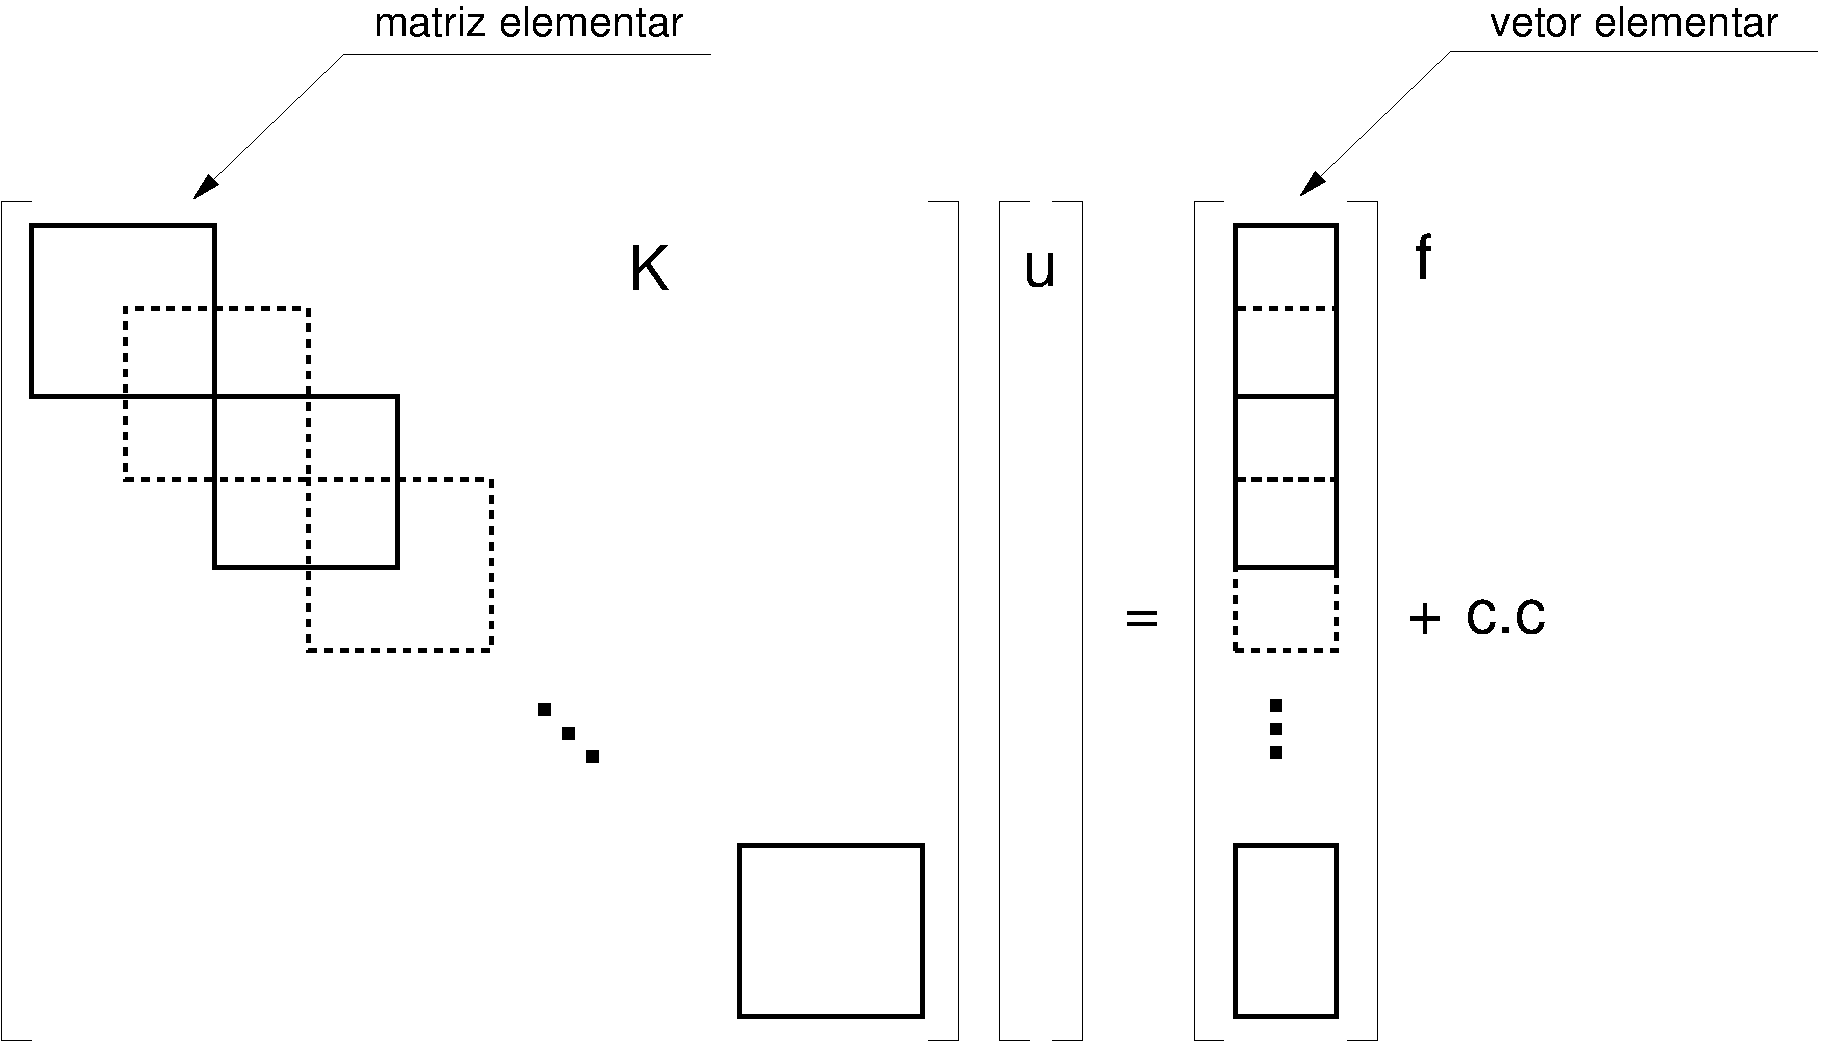
\includegraphics[scale=0.4]{figs/sistema.pdf}
		\caption[Sistema linear do método de elementos finitos]
		{Sistema linear resultante da discretização pelo método 
		de elementos finitos}
	\label{fig:sistema}
\end{figure}

\noindent e a solução do sistema linear fornece os valores da incógnita
$u$ nos nós dos elementos da malha.

A utilização do método de elementos finitos vem se tornando cada vez
mais frequente na indústria, na educação e na pesquisa. A reutilização
de código na forma de módulos e bibliotecas é uma grande aliada ao
desenvolvimento de grandes projetos, uma vez definida a base do código
(montagem de matrizes e vetores, solução do sitema linear), uma mudança
na geometria e nas condições de contorno do problema altera o tipo de
problema físico estudado, representando aproximadamente 10\% de
modificações no código numérico.   


\typeout{ ****************** End of file mef.tex ****************** }

